% The declaration of the document class:

% The second line here, i.e.
%
% \documentclass[a4paper]{article}  
%
% is a standard LaTeX document class declaration: 
% we say what kind of document we are making in curly brackets, 
% and specify any options in square brackets.
\documentclass[a4paper]{article}

\usepackage[T1]{fontenc}
\usepackage[utf8]{inputenc}
\usepackage[english]{babel}

% The following package allows us to define our own macros
% through "\LetLtxMacro\ourName\originalName"
\usepackage{letltxmacro}
\usepackage{csquotes}

% Adds vertical space between paragraphs, i.e. a clean linebreak
\usepackage{parskip} 

% Used for typesetting ordinary math
\usepackage{amsmath}

% These packages enables other useful math commands
\usepackage{amssymb}
\usepackage{amsthm}
\usepackage{amsfonts}

\usepackage{letltxmacro}
\LetLtxMacro\tt\texttt

\usepackage{graphicx}

% Allows us to use syntax highlighting on included files an
% in an inline fashion.
\usepackage{minted}

% Ignore syntax errors - the minted lexer is not perfect (MATLAB only)
\makeatletter
\expandafter\def\csname PYGdefault@tok@err\endcsname{\def\PYGdefault@bc##1{{\strut ##1}}}
\makeatother

% The package offers the command \DeclareFloatingEnvironment, which
% the user may use to define new floating environments which behave
% like the LaTeX standard foating environments figure and table.
\usepackage{newfloat}

% Improves the interface for defining floating objects such as figures
% and tables. You can define your own floats and improve the
% behaviour of the old ones.  
% 
% The package also provides the "H" float modifier option, which
% puts figures exactly where they are included as opposed to being
% placed where LaTeX deems as the most appropriate position
\usepackage{float} 
\floatplacement{figure}{H} % Set the H option globally

% Creates the Listing environment whereby you may specify fontsizes
% et al. when using \lstlisting
\usepackage{listings}
\usepackage{mips} % Load in the MIPS keywords

% Teach autoref how to reference listings
\providecommand*{\listingautorefname}{Listing} 

% Disallow the placement of the listing environment to be moved by LaTeX
\floatplacement{listing}{H}

\usepackage{xcolor}

\definecolor{keyword}{HTML}{A71D5D}
\definecolor{ident}{HTML}{333333}
\definecolor{background}{HTML}{F7F7F7}
\definecolor{registers}{HTML}{0086B3}

\lstset{
  aboveskip=20pt,                     % Vertical space above the listing
  belowskip=10pt,                     % Vertical space below the listing
  breaklines=true,                    % sets automatic line breaking
  basicstyle=\ttfamily,
  extendedchars=true,
  tabsize=2,
  columns=fixed,
  showstringspaces=false,
  captionpos=b,                       % sets the caption-position to bottom
  %
  % Insert a red arrow to highlight line-continuations
  postbreak=\raisebox{0ex}[0ex][0ex]{\ensuremath{\color{red}\hookrightarrow\space}},
}

\lstdefinestyle{mips_lst}{
  frame=trbl,
  language={[mips]Assembler},
  framesep=4pt,
  keywordstyle=\color{keyword},       % Keyword coloring
  identifierstyle=\lst@ifdisplaystyle\color{registers}\fi,
  backgroundcolor=\color{background},
}{}

\lstdefinestyle{semantics_lst}{
  aboveskip=2\medskipamount,
  belowskip=\medskipamount,
  mathescape=true, 
}{}

\usepackage[flushmargin]{footmisc} % Footnote position

\usepackage{hyperref}
\hypersetup{
  colorlinks = true, % Colours links instead of ugly boxes
  urlcolor = blue, % Colour for external hyperlinks
  linkcolor = blue, % Colour of internal links
  citecolor = red % Colour of citations
}

% Used to get the last page of the document, used in our document headers
\usepackage{lastpage}

% Specify date format
\usepackage[yyyymmdd]{datetime}
\renewcommand\dateseparator{-} % Separate date tokens with a "-"

\usepackage{booktabs}

% Use fancy document headers
\usepackage{fancyhdr}
\usepackage{tikz}
\usepackage{minted}
%\newcommand{\mij}[1]{\mintinline{java}{#1}}

\usetikzlibrary{
  matrix,
  positioning,
  shapes.geometric
}

\newcommand{\shamt}{\texttt{shamt}}
\newcommand{\funct}{\texttt{funct}}
\newcommand{\opcode}{\texttt{opcode}}
\newcommand{\rd}{\texttt{rd}}
\newcommand{\rs}{\texttt{rs}}
\newcommand{\rt}{\texttt{rt}}
\newcommand{\PC}{\texttt{PC}}

\usepackage{microtype}

\usepackage{varwidth}

% An environment for nice looking quotes
\makeatletter
\newenvironment{chapquote}[2][2em]
  {\setlength{\@tempdima}{#1}%
    \def\chapquote@author{#2}%
    \parshape 1 \@tempdima \dimexpr\textwidth-2\@tempdima\relax}
  {\par\normalfont\hfill\ \chapquote@author\hspace*{\@tempdima}\par}
  \makeatother

%
% BibLaTeX
%
% Great reference system
% Documentation:
% http://mirrors.ctan.org/macros/latex/contrib/biblatex/doc/biblatex.pdf
%___________________________________________________________
\usepackage[style = ieee, urldate =comp, backend=bibtex]{biblatex}
\addbibresource{references.bib}

\renewcommand\dateseparator{-}

\newcommand{\department}{Department of Computing Science}
\newcommand{\university}{Ume\aa\ University}

\newcommand{\authors}{Filip Allberg (\tt{filip@cs.umu.se}) \\
                      Jonathan Westin (\tt{jwestin@cs.umu.se})}
\author{\authors}
\newcommand{\coursename}{Computer Organization and Architecture}
\newcommand{\coursecode}{5DV118}
\newcommand{\instructor}{Thomas Johansson}

\pagestyle{fancy}
% Header settings
\fancyhead[R]{\thepage(\pageref{LastPage})}
\fancyheadoffset[L,R]{12mm}
\fancyhead[L]{\coursename{}: \titlename{} \\ \authors{}}
\fancyfoot[L,R,C]{}


\newcommand{\titlename}{MIPS32 Simulator}
\title{\titlename}

\begin{document}

\begin{titlepage}
\maketitle

\fancyfoot{}

\thispagestyle{fancy}
\headheight 35pt

\lhead{\small \department{} \\
\university{}} % These two are also defined in config.sty

\rhead{\small \today} %date

\cfoot{\coursename{} \coursecode{} HT16, 7.5 hp\\
Supervisor(s): \instructor{}}

\end{titlepage}


\tableofcontents
\clearpage

\section{Introduction}

In the MIPS32 architecture, all machine instructions are represented
as 32-bit numbers. This article presents a MIPS32-decompiler that,
when passed 32-bit numbers which either partially or completely
represent MIPS32 instructions yields a series of different
representations of the same instruction.

MIPS32 instructions are to be read from a file with numbers either in
decimal or hexadecimal form. For each number in the input file, the
disassembler will produce the following:

\begin{itemize}
  \item The number from the input file.
  \item The format of the instruction (R, I, or J).
  \item The decomposed representation in decimal.
  \item The decomposed representation in hexadecimal.
  \item The representation of the instruction in mnemonic format,
    using register abbreviations wherever possible (e.g.,
    \texttt{\$t0} instead of \texttt{\$8}) and using decimal numbers
    whenever actual numbers are necessary.
\end{itemize}

In the following subsections an introduction of the terminology used
throughout this document is provided. Afterwards you may refer to this
section again if any of the above requirements seem foreign to you.

The rest of the document will be dedicated to a high-level description
of this solution accompanied with a guide on how to compile and run
the software.

The appendix contains an overview of all those instructions that the
decompiler is capable of comprehending.

\subsection{Terminology}

According to Aho et al.\cite{Aho:2006:CPT:1177220} a \emph{compiler}
is a program that can read a program in one language --- the
\emph{source} language -- and translates it into an equivalent program
in another language -- the \emph{target} language; see
Fig.~\ref{fig:compiler}.

\begin{figure}[H]
  \centering
  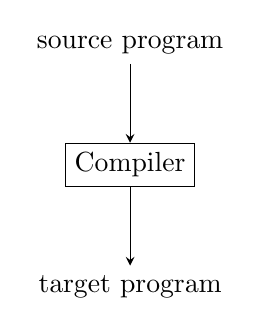
\begin{tikzpicture}[>=stealth]
  % Draw the labelled box. ``compiler'' is its label, and how
  % it is referred to within this TikZ picture. Its displayed
  % text is ``Compiler''. I.e. generically we'd write
  %
  % \node [draw] (nodelabel) {some text};
  %
  \node [draw] (compiler) {Compiler};

  % Create an input node, with the text ``source program'' 
  % which is above the box named ``compiler'', see above.
  \node [above=of compiler] (input) {source program};

  % Create an output node, with the text ``target program'' 
  % which is below the box named ``compiler'', see above.
  \node [below=of compiler] (output) {target program};

  % Draw an arrow _from_ the input node, to the compiler node.
  \draw [->] (input) -- (compiler);

  % Draw an array _from_ the compiler node to the output node.
  \draw [->] (compiler) -- (output);
\end{tikzpicture}

  \caption{A compiler}
  \label{fig:compiler}
\end{figure}

Conversely, a \emph{decompiler} is also a that performs the reverse
operation of a compiler. It too, is a compiler. Commonly one views a
compiler as a translator from a high-level human-readable source
language into a low-level machine-readable language, similarly a
decompiler translates in the opposite direction; see
Fig. \ref{fig:decompiler}. 

The two exhibit a chiral relation to one another, i. e. that they are
mirrored images of each other in terms of functionality, but they are
not themselves identical.

\begin{figure}[H]
  \centering
  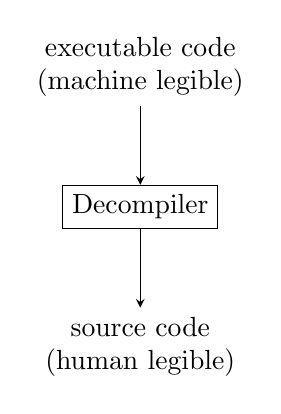
\begin{tikzpicture}[>=stealth]
  \node [draw] (decompiler) {Decompiler};
  \node [above=of decompiler, align=center] (input) {executable code \\ (machine legible)};
  \node [below=of decompiler, align=center] (output) {source code \\ (human legible)};
  \draw [->] (input) -- (decompiler);
  \draw [->] (decompiler) -- (output);
\end{tikzpicture}

  \caption{A decompiler}
  \label{fig:decompiler}
\end{figure}

In this assignment the decompiler must be able to translate from the
machine-readable language of 32-bit numbers representing MIPS32
instructions to the human-readable target language described in the
introduction. See \ref{fig:mipsdecompiler}

\begin{figure}[H]
  \centering
  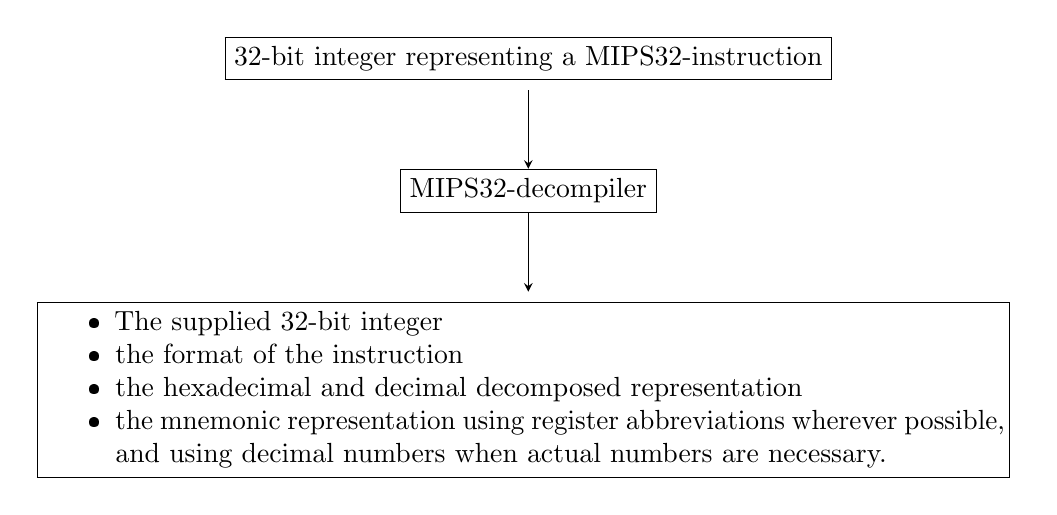
\begin{tikzpicture}[>=stealth]
  \node [draw] (decompiler) {MIPS32-decompiler};
  \node [above=of decompiler, align=center] (input) {\framebox{32-bit integer representing a MIPS32-instruction}};
  \node [below=of decompiler, align=center] (output) {
    \framebox{\begin{varwidth}{\linewidth}\begin{itemize}
          \item The supplied 32-bit integer
          \item the format of the instruction
          \item the hexadecimal and decimal decomposed representation
          \item the mnemonic representation using register
            abbreviations wherever possible, and using decimal numbers
            when actual numbers are necessary.
    \end{itemize}\end{varwidth}}
  };
  \draw [->] (input) -- (decompiler);
  \draw [->] (decompiler) -- (output);
\end{tikzpicture}

  \caption{Our MIPS32-decompiler}
  \label{fig:mipsdecompiler}
\end{figure}

\ref{fig:entrypointdecompiler} describes the programs entry-point into the
decompilation of an instruction.

\begin{figure}[H]
  \centering
  \begin{tikzpicture}[>=stealth]
  \node [draw] (compiler) {\mintinline{java}{Instruction.fromInteger}};
  \node [above=of compiler] (input) {32-bit integer (\mintinline{java}{int})};
  \node [below=of compiler] (output) {\mintinline{java}{Instruction}};
  \draw [->] (input) -- (compiler);
  \draw [->] (compiler) -- (output);
\end{tikzpicture}

  \caption{Entry point for our decompiler}
  \label{fig:entrypointdecompiler}
\end{figure}

\section{Simulation}\label{sec:simulation}

A \emph{simulator} is a system that behaves \emph{similar} to another
system, but is implemented in a different way. The simulator provides
the the same --- or the subset of the same --- behaviour of the sytem
being simulated. As in, the simulator may or may not enforce all of
the rules imposed by the original system. This is in contrast to an
\emph{emulator} that exhibits the same \emph{exact} behaviour, as the
emulator completely replicates the system being
emulated,\footnote{Going so far as having binary compatible with the
  emulated system's inputs and outputs} albeit operating in a
different environment.

With respect to our simulator the goal is to execute a MIPS32 assembly
program and modifying the processor state as an effect of each
executed instruction. 

This means that the processor registers, program counter, data- and
instruction memory is all affected, together with all other
``hardware''. Our software parses the program in an
instruction-by-instruction basis and allows each instruction to alter
the processor state. Each instruction is decoded, and the associated
operation is subsequently performed;
\autoref{sec:implementation-requirements} outlines all of the
behaviours our simulation is expected to exhibit.

In the context of our single-cycle implementation our datapath
contains all the functional units specified in
\autoref{sec:simulation-requirements} with the additions of
some multiplexors.


\input{requirements.tex}
\section{Technical background}

In this section we will introduce MIPS, juxtapose the two instruction
set architectures RISC and CISC, and provide a cursory overview --- as
well as reviewing (briefly) --- the MIPS instruction set in
preparation for the rest of this document.

\subsection{MIPS, RISC and CISC}

MIPS (originally an acronym for Microprocessor without Interlocked
Pipeline Stages) is a ``reduced instruction set computer'' (RISC), as
opposed to a ``complex instruction set computer'' (CISC), instruction
set architecture (ISA) developed by MIPS Technologies (formerly MIPS
Computer Systems, Inc.). Meanwhile, RISC is a [design] concept
developed at IBM, Stanford and UC Berkeley in the late 1970s and early
1980s to overcome the typical deficiencies of CPUs of the 1970s
 \cite{CNS:RISC-Architecture}\cite{Stokes:1999:RISCvsCISC}. Specifically the deficiencies
experienced with CISC ISAs.
% This ending sentence is iffy.

We find that RISC offers two expressly \emph{practical} advantages
over CISC. Per definition RISC has fewer and simpler instructions,
and in 2001 Bart Trzynadlowski showed that the \tt{tst}, \tt{beq},
\tt{bne}, \tt{move}, \tt{cmp}, \tt{cmpi} make up more
than 70\% of all instructions executed on a Motorola
M68K.\footnote{While many associate Motorola with cell-phones, and
  rightfully so, the M68K was a 32-bit CISC microprocessor that were
  used in calculators, UNIX workstations, and the Space Shuttle}
\cite{Trzynadlowski:2001:68k} 

The idea of the ``quantitative approach to computer design''
\cite{Patterson:2008:COD:1502247} is to make the common case fast,
which in itself is one of the four corner-stone design principles
behind RISC.\footnote{The remaining three are ``Simplicity favors
  regularity'', ``Smaller is faster'', and ``Good design demands
  compromises''.\cite{Irwin:CSE331W02.11:2007:PSU}}

A CISC-architecture requires the use of a microcode interpreter but by
removing complex instructions from the instruction set the interpreter
is made obsolete, as decoding is easier. This effect is compounded
further if all of the instructions have the same width. All remaining
instructions can be executed in one clock cycle, which makes
pipelining and superscalar execution ``easy''. The design is a lot
simpler, work has been moved from hardware to software.

\textbf{A load/store architecture and more registers}

As the RISC architecture makes both the microcode interpreter and the
``complex instruction'' decoder redundant we can use the transistors
otherwise occupied by the aforementioned two so that they may be used
for other purposes, for instance multiple ALUs, better pipelining
logic and many additional registers.

A CPU with more registers affords more operations to be performed on
its registers, alleviating the significant cost of memory accesses
resulting in greater performance. With RISC there cannot be any
implicit memory accesses, as there can be in CISC, hence the term
``load/store architecture'': all memory accesses are only possible
through load and store instructions; all other operations only work on
registers.

The time required for a program to execute is calculated using this
formula:

\begin{equation*}
\frac{\textrm{time}}{\textrm{program}} =
\frac{\textrm{time}}{\textrm{cycle}} \cdot
\frac{\textrm{cycles}}{\textrm{instruction}} \cdot
\frac{\textrm{instructions}}{\textrm{program}}
\end{equation*}

CISC CPUs keep the number of instructions per program low, while the
time/cycle is high.  Because RISC CPUs do not have complex
instructions, the number of instructions per program is higher, but
this is compensated by a lower number of cycles per instruction. 

Beyond its practical applications RISC is also well-suited for
academic excursions such as this one. With a smaller set of
instructions, all of equal width, it is arguably better suited as a
pedagogical teaching tool for understanding the internal operation of
a modern microprocessor.

\subsection{Instruction Encoding}

In the MIPS32 architecture, all machine instructions are represented
as 32-bit numbers. Throughout this document we will intermittently
dissect these 32-bits into various lengths. We regard the ``upper''
--- or equivalently the ``leftmost'' --- bits as the most significant
bits. Hence, we consider the bit order to be little endian.

In little endian bit notation we denote bit 0 as being the least
significant bit (LSB) and bit 31 as the most significant bit (MSB).

Then, for all MIPS32 instructions we have that the leftmost six bits,
31-26, forms the primary opcode. These bits constitute a field which
are referred to as the \tt{op} field of the instruction.
Depending on the value of the primary opcode there can be an extended
opcode in the rightmost six bits, i.e. bits 0 through 5.  These bits
are referred to as the \funct{} field.\footnote{The decoding of
  the \funct{} field provides details of the required operation
  to the \tt{ALU}.}

Ostensibly, the different fields a MIPS instruction should be divided
into is determined solely by the opcode. The manner in which the bits
are divvied up into fields depends on which instruction format that
the instruction has.

Regardless of the type of the instruction we have that the
\opcode{} field is the uppermost six bits of all MIPS
instructions. Opcode, short for ``operation code'', either identifies
a unique instruction or a \emph{set} of instructions.

While MIPS consists of over a 100 different instructions only 6 bits
are used for the \opcode{}, meaning that the
\opcode{}-field can only be used to differentiate between
$2^6=64$ instructions. 

For R-type instructions an additional 6 bits are used (\textbf{B5-0})
called the ``function'', which serves as a secondary opcode to
identify the instruction. I.e. the tuple

\begin{equation*}
(\opcode{},\ \funct{})
\end{equation*}

is sufficient to \emph{uniquely} identify an R-type instruction.

Other instructions, such as \texttt{bltzal}\footnote{Not an R-type
instruction}, is identified by the tuple

\begin{equation*}
(\opcode{}=1,\ \rt{}=16) \textrm{\hspace{1em}(Remark: base 10)}
\end{equation*}

The MIPS ISA groups its instructions into three
categories:\footnote{Some people consider floating-point and branching
  instructions to be their own respective categories} R-type, I-type, and J-type.

\subsubsection{R-type format}

R-type instructions refer to \emph{register} type instructions. These,
when encoded in machine code, are split into 6 fields of lengths 6, 5,
5, 5, 5, 6 respectively, see ~\autoref{fig:r-type-format-bit-fields}.

\begin{figure}[H]
  % Center the image on the page using makebox  
  \makebox[\textwidth][c]{
    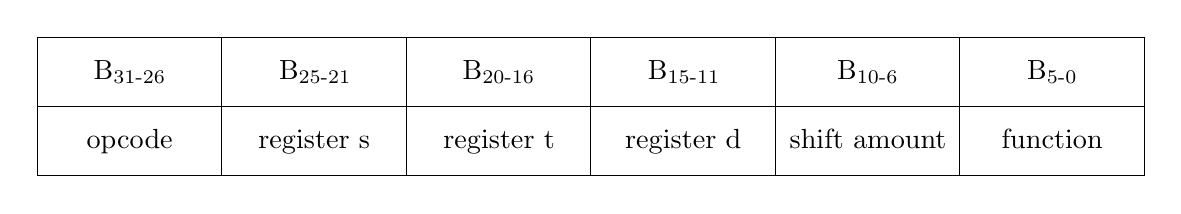
\begin{tikzpicture}[auto,
    every node/.style={rectangle, minimum height=2.5em, text centered, text width=6em, text height=1.5ex, text depth=.25ex},
    field/.style={draw}]
\matrix (m) [ampersand replacement=\&, column sep=-\pgflinewidth, row sep=-\pgflinewidth]
{
\node [field] {$\textrm{B}_{31\textrm{-}26}$}; \&
\node [field] {$\textrm{B}_{25\textrm{-}21}$}; \&
\node [field] {$\textrm{B}_{20\textrm{-}16}$}; \&
\node [field] {$\textrm{B}_{15\textrm{-}11}$}; \&
\node [field] {$\textrm{B}_{10\textrm{-}6}$}; \&
\node [field] {$\textrm{B}_{5\textrm{-}0}$}; \&
\\
\node [field] {opcode}; \&
\node [field] {register s}; \&
\node [field] {register t}; \&
\node [field] {register d}; \&
\node [field] {shift amount}; \&
\node [field] {function}; \&
\\
};
\end{tikzpicture}
%
  } 
  \caption{The bitfields of an R-type format instruction}
  \label{fig:r-type-format-bit-fields}
\end{figure}

For instance, \tt{add} is an R-type instruction, and in
its mnemonic form it looks like

\begin{lstlisting}[style=mips_lst]
add $rd, $rs, $rt
\end{lstlisting}
%$

where \tt{\$rd} refers to some register \tt{d}.

The semantics of the instruction is

\begin{lstlisting}[style=semantics_lst]
R[d] = R[s] + R[t]
\end{lstlisting}

where the addition is signed addition. Hence, \tt{\$rd} is the
target/destination register while the operands \tt{\$rs} and
\tt{\$rt} are the two source registers.\footnote{Notice that the
  mnemonic representation specifies the destination register
  \emph{first} followed by the two source registers but the the actual
  binary format stores the two source registers first, then the
  destination register.}

Certain R-type instructions places certain constraints on its
constituent fields beyond the value of the opcode and the funct
field. Several instructions are only valid if \shamt{} is set to
0, and specifies the shift amount used by shifting instructions such
as \tt{sll} (shift left logical). \tt{clo} (count leading
zeroes) expects both \shamt{} and \tt{rt} to be equal to
zero, and meanwhile \tt{div} (divide with overflow) expects
\rd{} and \shamt{} to be zero.

\subsubsection{I-type format}

I-type stands for "immediate type", and it is decomposed into four
fields. See ~\autoref{fig:i-type-format-bit-fields}.

\begin{figure}[H]
  \makebox[\textwidth][c]{
    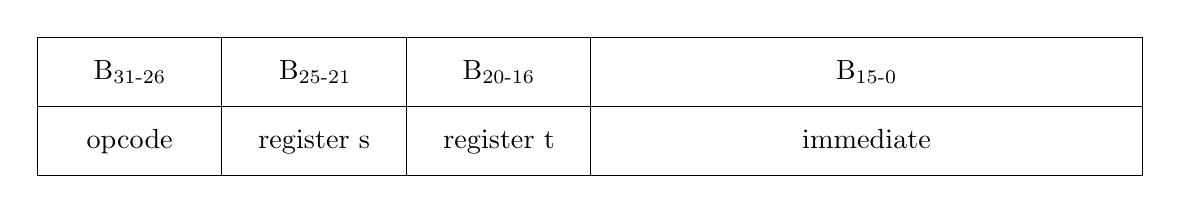
\begin{tikzpicture}[auto,
    every node/.style={rectangle, minimum height=2.5em, text centered, text width=6em, text height=1.5ex, text depth=.25ex},
    field/.style={draw, anchor=west}]
\matrix (m) [ampersand replacement=\&, column sep=-\pgflinewidth, row sep=-\pgflinewidth]
{
\node [field] {$\textrm{B}_{31\textrm{-}26}$}; \&
\node [field] {$\textrm{B}_{25\textrm{-}21}$}; \&
\node [field] {$\textrm{B}_{20\textrm{-}16}$}; \&
\node [field, text width=19.25em] {$\textrm{B}_{15\textrm{-}0}$}; \&
\\
\node [field] {opcode}; \&
\node [field] {register s}; \&
\node [field] {register t}; \&
\node [field, text width=19.25em] {immediate}; \&
\\
};
\end{tikzpicture}
%
  }
  \caption{The bitfields of an I-type format instruction}
  \label{fig:i-type-format-bit-fields}
\end{figure}

The prototypical I-type instruction in its mnemonic form looks as follows,

\begin{lstlisting}[style=mips_lst]
addi $rt, $rs, immed
\end{lstlisting}

In this case, \tt{\$rt} is the destination register, and
\tt{\$rs} is the \emph{only} source register.

The semantics of the \tt{addi} instruction is

\begin{lstlisting}[style=semantics_lst]
R[t] = R[s] + (IR$_{15})^{16}$ IR$_{15\textrm{-}0}$
\end{lstlisting}

where \tt{IR} refers to the instruction register, the register
where the current instruction is stored. \tt{(IR$_{15}$)$^{16}$}
means that bit \textbf{B15} of the instruction register (which is the
sign bit of the immediate value) is repeated 16 times. This is then
followed by \tt{IR$_{15\textrm{-}0}$}, which is the 16 bits of
the immediate value.

Basically, the semantics says to sign-extend the immediate value to 32
bits, add it (using signed addition) to register \tt{R[s]}, and store
the result in register \tt{\$rt}.

For an example,

\begin{lstlisting}[style=mips_lst]
addi $s1, $s2, 100
\end{lstlisting}
%$

stores the value of $(\tt{\$s2} + 100)$ in \tt{\$s1}.

\subsubsection{J-type format}

All jump instructions belong to the J-type format

J-type instructions refer to \emph{jump} type instructions. These,
when encoded in machine code, are split into 2 fields of lengths 6 and
26, respectively. See ~\autoref{fig:r-type-format-bit-fields}.

\begin{figure}[H]
  \makebox[\textwidth][c]{
    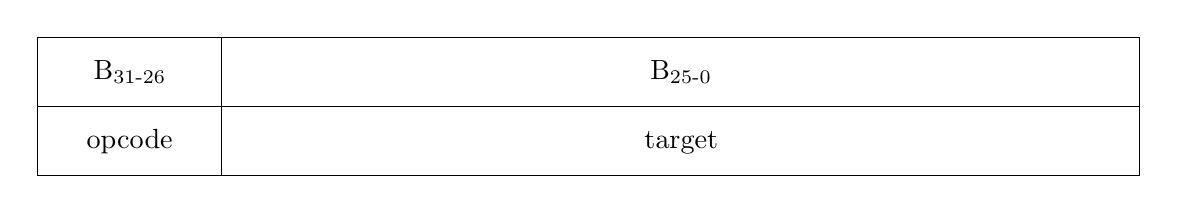
\begin{tikzpicture}[auto,
    every node/.style={rectangle, minimum height=2.5em, text centered, text width=6em, text height=1.5ex, text depth=.25ex},
    field/.style={draw}]
\matrix (m) [ampersand replacement=\&, column sep=-\pgflinewidth, row sep=-\pgflinewidth]
{
\node [field] {$\textrm{B}_{31\textrm{-}26}$}; \&
\node [field, text width=32.5 em] {$\textrm{B}_{25\textrm{-}0}$}; \&
\\
\node [field] {opcode}; \&
\node [field, text width=32.5 em] {target}; \&
\\
};
\end{tikzpicture}
%
  }
  \caption{The bitfields of an J-type format instruction}
  \label{fig:j-type-format-bit-fields}
\end{figure}

For an example the instruction \tt{j} is J-type instruction, and in
its mnemonic form as follows,

\begin{lstlisting}[style=mips_lst]
j target
\end{lstlisting}
%$

\tt{j} is the archetypal jump instruction. In ~\autoref{lst:jump}
``\PC{}'' stands for ``program counter''. The program counter stores
the current address of the instruction that is \emph{currently}
being executed.

In effect, what the \tt{j} instruction does, as shown in
~\autoref{lst:jump}, is re-assign the \PC{} the 32-bit address given
by the upper 4 bits of the \PC{} followed by the 26-bits making up the
target, followed by two zeroes.

\begin{lstlisting}[style=semantics_lst, label={lst:jump}]
PC := PC$_{31\textrm{-}28}$ IR$_{25\textrm{-}0}$ 00
\end{lstlisting}


\subsubsection{MIPS Register Naming and Usage Convention}

Within the MIPS32 architecture there are 32 general-purpose registers,
see \autoref{table:mips-register-naming-and-usage-convention}. The
registers when written out, are preceded by a ``\tt{\$}''.  We use
two formats for addressing a particular register, e.g. \tt{\$0}
through \tt{\$31}. Or, using their equivalent mnemonic
representations, for instance \tt{\$t1}. Both formats may be used
interchangeably in the assembly language.

\begin{table}[H]
\centering
\begin{tabular}{lll}
\toprule
Mnemonic & Register Number & Usage                                                     \\
\midrule
\tt{\$zero}                & 0       & constant 0                                      \\
\tt{\$at}                  & 1       & reserved for assembler                          \\
\tt{\$v0} - \tt{\$v1}      & 2 - 3   & expression evaluation and results of a function \\
\tt{\$a0} - \tt{\$a3}      & 4 - 7   & argument 1 through 4                            \\
\tt{\$t0} - \tt{\$t7}      & 8 - 15  & temporary (not preserved across call)           \\
\tt{\$s0} - \tt{\$s7}      & 16 - 23 & saved temporary (preserved across call          \\
\tt{\$t8} - \tt{\$t9}      & 24 - 25 & temporary (not preserved across call)           \\
\tt{\$k0} - \tt{\$k1}      & 26 - 27 & reserved for OS kernel                          \\
\tt{\$gp}                  & 28      & pointer to global area                          \\
\tt{\$sp}                  & 29      & stack pointer                                   \\
\tt{\$fp}                  & 30      & frame pointer                                   \\
\tt{\$ra}                  & 31      & return address (used by function call)          \\
\bottomrule
\end{tabular}
\caption{MIPS register naming and usage convention}
\label{table:mips-register-naming-and-usage-convention}
\end{table}

\subsection{Instruction Encoding}

In the MIPS32 architecture, all machine instructions are represented
as 32-bit numbers. Throughout this document we will intermittently
dissect these 32-bits into various lengths. We regard the ``upper''
--- or equivalently the ``leftmost'' --- bits as the most significant
bits. Hence, we consider the bit order to be little endian.

In little endian bit notation we denote bit 0 as being the least
significant bit (LSB) and bit 31 as the most significant bit (MSB).

Then, for all MIPS32 instructions we have that the leftmost six bits,
31-26, forms the primary opcode. These bits constitute a field which
are referred to as the \tt{op} field of the instruction.
Depending on the value of the primary opcode there can be an extended
opcode in the rightmost six bits, i.e. bits 0 through 5.  These bits
are referred to as the \funct{} field.\footnote{The decoding of
  the \funct{} field provides details of the required operation
  to the \tt{ALU}.}

Ostensibly, the different fields a MIPS instruction should be divided
into is determined solely by the opcode. The manner in which the bits
are divvied up into fields depends on which instruction format that
the instruction has.

Regardless of the type of the instruction we have that the
\opcode{} field is the uppermost six bits of all MIPS
instructions. Opcode, short for ``operation code'', either identifies
a unique instruction or a \emph{set} of instructions.

While MIPS consists of over a 100 different instructions only 6 bits
are used for the \opcode{}, meaning that the
\opcode{}-field can only be used to differentiate between
$2^6=64$ instructions. 

For R-type instructions an additional 6 bits are used (\textbf{B5-0})
called the ``function'', which serves as a secondary opcode to
identify the instruction. I.e. the tuple

\begin{equation*}
(\opcode{},\ \funct{})
\end{equation*}

is sufficient to \emph{uniquely} identify an R-type instruction.

Other instructions, such as \texttt{bltzal}\footnote{Not an R-type
instruction}, is identified by the tuple

\begin{equation*}
(\opcode{}=1,\ \rt{}=16) \textrm{\hspace{1em}(Remark: base 10)}
\end{equation*}

The MIPS ISA groups its instructions into three
categories:\footnote{Some people consider floating-point and branching
  instructions to be their own respective categories} R-type, I-type, and J-type.

\subsubsection{R-type format}

R-type instructions refer to \emph{register} type instructions. These,
when encoded in machine code, are split into 6 fields of lengths 6, 5,
5, 5, 5, 6 respectively, see ~\autoref{fig:r-type-format-bit-fields}.

\begin{figure}[H]
  % Center the image on the page using makebox  
  \makebox[\textwidth][c]{
    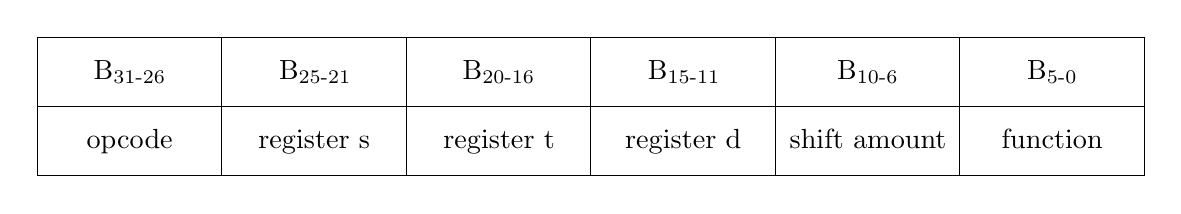
\begin{tikzpicture}[auto,
    every node/.style={rectangle, minimum height=2.5em, text centered, text width=6em, text height=1.5ex, text depth=.25ex},
    field/.style={draw}]
\matrix (m) [ampersand replacement=\&, column sep=-\pgflinewidth, row sep=-\pgflinewidth]
{
\node [field] {$\textrm{B}_{31\textrm{-}26}$}; \&
\node [field] {$\textrm{B}_{25\textrm{-}21}$}; \&
\node [field] {$\textrm{B}_{20\textrm{-}16}$}; \&
\node [field] {$\textrm{B}_{15\textrm{-}11}$}; \&
\node [field] {$\textrm{B}_{10\textrm{-}6}$}; \&
\node [field] {$\textrm{B}_{5\textrm{-}0}$}; \&
\\
\node [field] {opcode}; \&
\node [field] {register s}; \&
\node [field] {register t}; \&
\node [field] {register d}; \&
\node [field] {shift amount}; \&
\node [field] {function}; \&
\\
};
\end{tikzpicture}
%
  } 
  \caption{The bitfields of an R-type format instruction}
  \label{fig:r-type-format-bit-fields}
\end{figure}

For instance, \tt{add} is an R-type instruction, and in
its mnemonic form it looks like

\begin{lstlisting}[style=mips_lst]
add $rd, $rs, $rt
\end{lstlisting}
%$

where \tt{\$rd} refers to some register \tt{d}.

The semantics of the instruction is

\begin{lstlisting}[style=semantics_lst]
R[d] = R[s] + R[t]
\end{lstlisting}

where the addition is signed addition. Hence, \tt{\$rd} is the
target/destination register while the operands \tt{\$rs} and
\tt{\$rt} are the two source registers.\footnote{Notice that the
  mnemonic representation specifies the destination register
  \emph{first} followed by the two source registers but the the actual
  binary format stores the two source registers first, then the
  destination register.}

Certain R-type instructions places certain constraints on its
constituent fields beyond the value of the opcode and the funct
field. Several instructions are only valid if \shamt{} is set to
0, and specifies the shift amount used by shifting instructions such
as \tt{sll} (shift left logical). \tt{clo} (count leading
zeroes) expects both \shamt{} and \tt{rt} to be equal to
zero, and meanwhile \tt{div} (divide with overflow) expects
\rd{} and \shamt{} to be zero.

\subsubsection{I-type format}

I-type stands for "immediate type", and it is decomposed into four
fields. See ~\autoref{fig:i-type-format-bit-fields}.

\begin{figure}[H]
  \makebox[\textwidth][c]{
    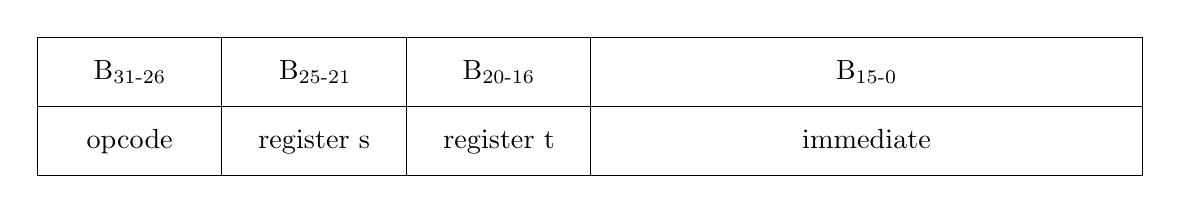
\begin{tikzpicture}[auto,
    every node/.style={rectangle, minimum height=2.5em, text centered, text width=6em, text height=1.5ex, text depth=.25ex},
    field/.style={draw, anchor=west}]
\matrix (m) [ampersand replacement=\&, column sep=-\pgflinewidth, row sep=-\pgflinewidth]
{
\node [field] {$\textrm{B}_{31\textrm{-}26}$}; \&
\node [field] {$\textrm{B}_{25\textrm{-}21}$}; \&
\node [field] {$\textrm{B}_{20\textrm{-}16}$}; \&
\node [field, text width=19.25em] {$\textrm{B}_{15\textrm{-}0}$}; \&
\\
\node [field] {opcode}; \&
\node [field] {register s}; \&
\node [field] {register t}; \&
\node [field, text width=19.25em] {immediate}; \&
\\
};
\end{tikzpicture}
%
  }
  \caption{The bitfields of an I-type format instruction}
  \label{fig:i-type-format-bit-fields}
\end{figure}

The prototypical I-type instruction in its mnemonic form looks as follows,

\begin{lstlisting}[style=mips_lst]
addi $rt, $rs, immed
\end{lstlisting}

In this case, \tt{\$rt} is the destination register, and
\tt{\$rs} is the \emph{only} source register.

The semantics of the \tt{addi} instruction is

\begin{lstlisting}[style=semantics_lst]
R[t] = R[s] + (IR$_{15})^{16}$ IR$_{15\textrm{-}0}$
\end{lstlisting}

where \tt{IR} refers to the instruction register, the register
where the current instruction is stored. \tt{(IR$_{15}$)$^{16}$}
means that bit \textbf{B15} of the instruction register (which is the
sign bit of the immediate value) is repeated 16 times. This is then
followed by \tt{IR$_{15\textrm{-}0}$}, which is the 16 bits of
the immediate value.

Basically, the semantics says to sign-extend the immediate value to 32
bits, add it (using signed addition) to register \tt{R[s]}, and store
the result in register \tt{\$rt}.

For an example,

\begin{lstlisting}[style=mips_lst]
addi $s1, $s2, 100
\end{lstlisting}
%$

stores the value of $(\tt{\$s2} + 100)$ in \tt{\$s1}.

\subsubsection{J-type format}

All jump instructions belong to the J-type format

J-type instructions refer to \emph{jump} type instructions. These,
when encoded in machine code, are split into 2 fields of lengths 6 and
26, respectively. See ~\autoref{fig:r-type-format-bit-fields}.

\begin{figure}[H]
  \makebox[\textwidth][c]{
    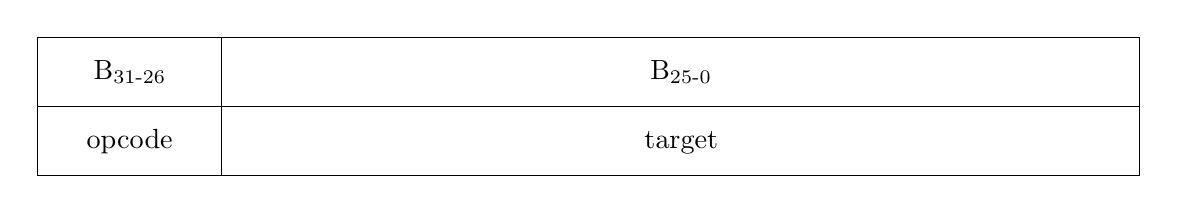
\begin{tikzpicture}[auto,
    every node/.style={rectangle, minimum height=2.5em, text centered, text width=6em, text height=1.5ex, text depth=.25ex},
    field/.style={draw}]
\matrix (m) [ampersand replacement=\&, column sep=-\pgflinewidth, row sep=-\pgflinewidth]
{
\node [field] {$\textrm{B}_{31\textrm{-}26}$}; \&
\node [field, text width=32.5 em] {$\textrm{B}_{25\textrm{-}0}$}; \&
\\
\node [field] {opcode}; \&
\node [field, text width=32.5 em] {target}; \&
\\
};
\end{tikzpicture}
%
  }
  \caption{The bitfields of an J-type format instruction}
  \label{fig:j-type-format-bit-fields}
\end{figure}

For an example the instruction \tt{j} is J-type instruction, and in
its mnemonic form as follows,

\begin{lstlisting}[style=mips_lst]
j target
\end{lstlisting}
%$

\tt{j} is the archetypal jump instruction. In ~\autoref{lst:jump}
``\PC{}'' stands for ``program counter''. The program counter stores
the current address of the instruction that is \emph{currently}
being executed.

In effect, what the \tt{j} instruction does, as shown in
~\autoref{lst:jump}, is re-assign the \PC{} the 32-bit address given
by the upper 4 bits of the \PC{} followed by the 26-bits making up the
target, followed by two zeroes.

\begin{lstlisting}[style=semantics_lst, label={lst:jump}]
PC := PC$_{31\textrm{-}28}$ IR$_{25\textrm{-}0}$ 00
\end{lstlisting}


\subsubsection{Example: Numeric decoding}

Consider the machine-language MIPS32 instruction \tt{0x71014802}.
Depending on the format of the instruction it decomposes into fields
varying lengths.

Recall that for all numbers in the MIPS32 instruction set the leftmost
six bits always represent the opcode for the instruction. The opcode
alone is not always sufficient to identify the particular instruction,
\emph{but} it is always sufficient to identify the format of the
instruction.

The leftmost six bits of \tt{0x71014802} is \tt{0x1c}. It is
\emph{known} that this number corresponds to a set of instructions in
the R-type format. The format specifies into which fields the 32-bit
decomposes into. The number of bits composing each respective field is
given in the bottom row of ~\autoref{fig:r-decomposed},

\begin{figure}[H]
\centering
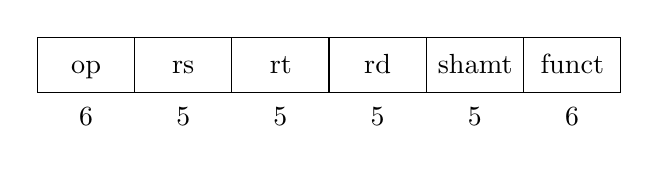
\begin{tikzpicture}[node distance=1em]

\matrix (decomposed-representation) [
  matrix of nodes,
  row sep=0.2em,
  column sep=-\pgflinewidth,
  row 1/.style={
    nodes={
      rectangle, 
      draw, 
      text centered,
          text width=10mm,
      anchor=base,
      text height=.8em,text depth=.2em,minimum size=7mm
    }
  }
] {
op & rs & rt & rd & shamt & funct \\
6 & 5 & 5 & 5 & 5 & 6 \\
};
\end{tikzpicture}

\caption{The length of each respective field for R-type format instructions}
\label{fig:r-decomposed}
\end{figure}

Decomposing \tt{0x71014802} into the fields shown in
\autoref{fig:r-decomposed} yields \tt{rs=8}, \tt{rt=1}, \tt{rd=9},
\tt{shamt=0}, and \tt{funct=2}. The \emph{decomposed representation}
of this instruction in hexadecimal form is thus \tt{[0x1c 8 1 9 0
  2]}.\footnote{The corresponding \emph{decimal representation} is
  \tt{[28 8 1 9 0 2]}}

To identify the particular instruction represented by \tt{0x71014802}
the \funct{} field must be consulted. Pairing the opcode, \tt{0x1c}
and the value in the \funct{} field uniquely identifies the
instruction a \tt{mul} instruction; see \autoref{fig:mul-decomposed}.

\begin{figure}[H]
  \centering
  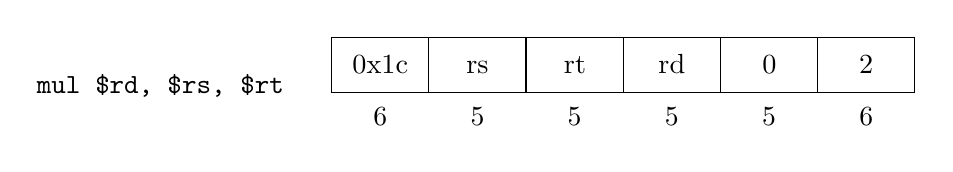
\begin{tikzpicture}[node distance=1em]
\matrix (decomposed-representation) [
  matrix of nodes,
  row sep=0.2em,
  column sep=-\pgflinewidth,
  row 1/.style={
    nodes={
      rectangle, 
      draw, 
      text centered,
          text width=10mm,
      anchor=base,
      text height=.8em,text depth=.2em,minimum size=7mm
    }
  }
] {
0x1c & rs & rt & rd & 0 & 2 \\
6 & 5 & 5 & 5 & 5 & 6 \\
};
\node [left=of decomposed-representation] (mnemonic-representation) {\texttt{mul \$rd, \$rs, \$rt}};
\end{tikzpicture}

  \caption{Decomposition and mnemonic representation of \tt{mul}}
  \label{fig:mul-decomposed}
\end{figure}

Earlier we determined the fields \tt{rs}, \tt{rt} and \rd{} to have
the addresses 8, 1, and 9, respectively. In MIPS registers are named,
following the convention shown in
\autoref{table:mips-register-naming-and-usage-convention}

Replacing the numerical values of \tt{rs}, \tt{rt} and \rd{}, with
their named counterparts yields the \emph{mnemonic representation} of
the instruction to be

\begin{lstlisting}[style=mips_lst]
mul $t1, $t0, $at
\end{lstlisting}
%$

\subsubsection{Example: Mnemonic decoding}

The reverse operation, translating from a human-legible form to the
numerical form, is trivial. Given, of course, that you know the format
that the mnemonic form is in and any conditions pertaining to the
particular instruction. 

Take for instance \tt{div \$t2, \$t4}, given that we know its mnemonic
representation to be on the form

\begin{lstlisting}[style=mips_lst]
div $rs, $rt
\end{lstlisting}
%$

and that due to its nature both \shamt{} and \rd{} is both zero,
together with the fact that we know its opcode and \funct{}, trivially
we substitute all those values in together with the register
addresses. Together we get

\begin{figure}[H]
  \makebox[\textwidth][c]{
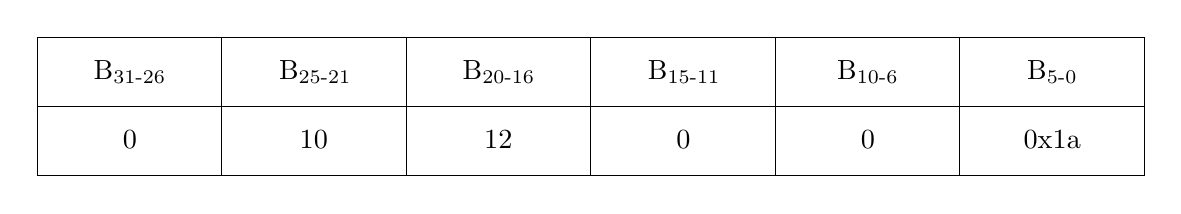
\begin{tikzpicture}[auto,
    every node/.style={rectangle, minimum height=2.5em, text centered, text width=6em, text height=1.5ex, text depth=.25ex},
    field/.style={draw}]
\matrix (m) [ampersand replacement=\&, column sep=-\pgflinewidth, row sep=-\pgflinewidth]
{
\node [field] {$\textrm{B}_{31\textrm{-}26}$}; \&
\node [field] {$\textrm{B}_{25\textrm{-}21}$}; \&
\node [field] {$\textrm{B}_{20\textrm{-}16}$}; \&
\node [field] {$\textrm{B}_{15\textrm{-}11}$}; \&
\node [field] {$\textrm{B}_{10\textrm{-}6}$}; \&
\node [field] {$\textrm{B}_{5\textrm{-}0}$}; \&
\\
\node [field] {0}; \&
\node [field] {10}; \&
\node [field] {12}; \&
\node [field] {0}; \&
\node [field] {0}; \&
\node [field] {0x1a}; \&
\\
};
\end{tikzpicture}
  }
\end{figure}

and the final translation step, and the resulting numerical
representation, is given by a sequence of bit-shift operations, in
this case the following will serve,\footnote{No operations are
  required for the zeroes.}\footnote{Notice that the shift amount (21,
  16) corresponds directly to the lower most bit of the respective fields (rs, rt)}

\begin{lstlisting}
(10 << 21) | (12 << 16) | 0x1a
\end{lstlisting}

which is equal to \tt{0x014c001a}.



\section{Usage and compilation}

We will now describe how to compile and use the supplied software, so
that you may experiment with it later when the solution is described.

The source code may be downloaded at the following two addresses,

\begin{center}
\url{https://github.com/leksak/kilobyte.git} \\
\url{git@github.com:leksak/kilobyte.git}
\end{center}

Or viewed in the following folder
\tt{\raise.17ex\hbox{$\scriptstyle\mathtt{\sim}$}filip/edu/kilobyte}
on the institution's network.

For the duration of this report the directory created by cloning
the repository is referred to as the \emph{root directory}.

\section{Compilation and usage}

In this section the compilation of the software is described as
is the usage of the software

\subsection{Compilation}

Navigate to the root directory of the project.

Whilst there execute the following command to compile the program:

\begin{lstlisting}[style=plain]
$ ./gradlew simulatorJar
\end{lstlisting}

In the \tt{build/libs} directory you will now find a file named
\tt{kilobyte-all-1.0-SNAPSHOT.jar} which you can run using \tt{java -jar
  kilobyte-all-1.0-SNAPSHOT.jar} given that you have Java 8 shown when running
\tt{java -version}.

\subsection{Usage}

When you first start the program you'll see a window displaying all
the constituent elements of the program that are available for user
display. In particular we observe in ~\autoref{fig:initial-gui} that
there is a panel to the left for the registers and the program counter
(PC), a panel to the right containing both instruction- and
datamemory, in the middle is a pane for displaying programs, and at
the bottom there is an additional panel displaying the values of all
of the control lines.

\begin{figure}[H]
  \centering
  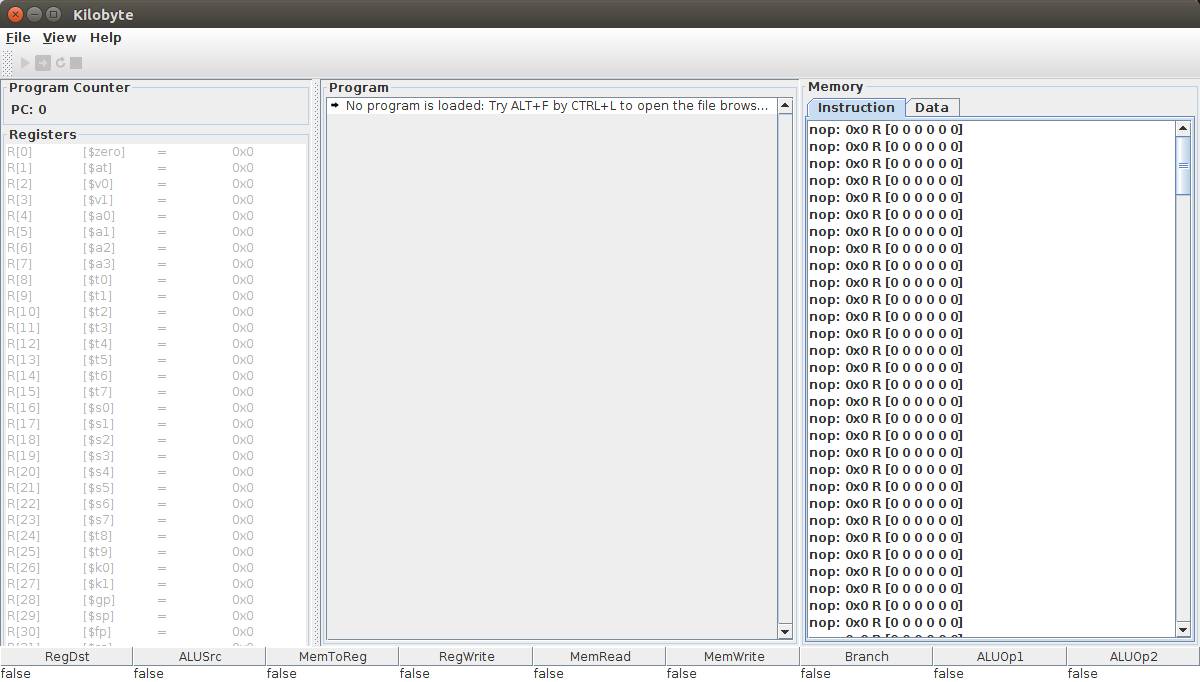
\includegraphics[width=\textwidth]{images/initial_gui.png} 
  \caption{Initial look} 
  \label{fig:initial-gui}
\end{figure}

Through the \emph{View} menu we can change the radix display for
different components in the interface. In
~\autoref{fig:change-radix-1} we see how the user can change the radix
display setting for the Data memory. In
~\autoref{fig:change-radix-1-result} we see the effect of applying the
operation as the hexadecimal prefix ``0x'' dissappears.

\begin{figure}[H]
  \centering
  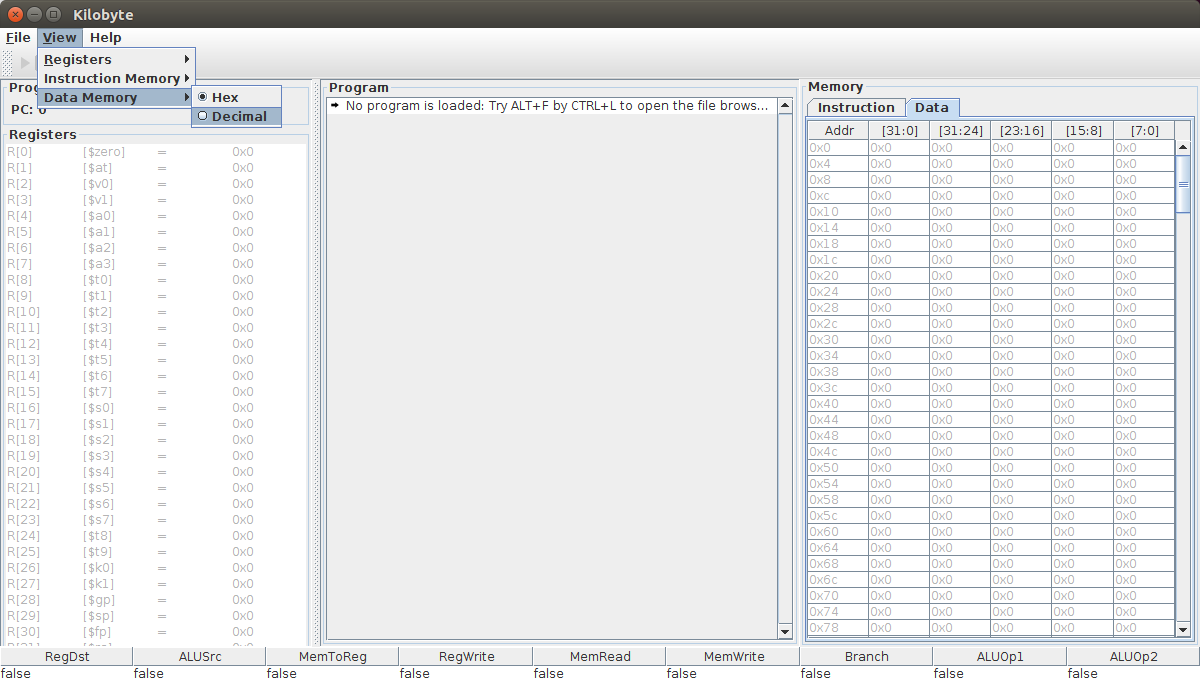
\includegraphics[width=\textwidth]{images/changing_data_memory_radix_to_dec.png} 
  \caption{Changing the data memory radix display setting to decimal} 
  \label{fig:change-radix-1}
\end{figure}

\begin{figure}[H]
  \centering
  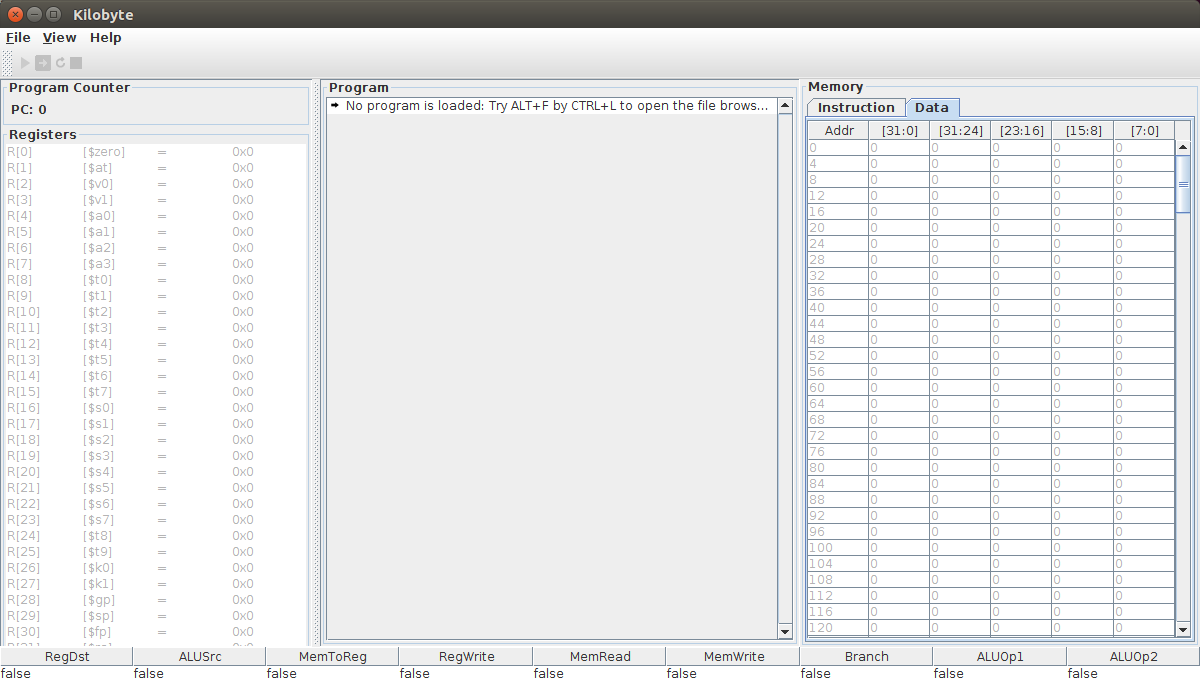
\includegraphics[width=\textwidth]{images/radix_display_result.png} 
  \caption{Changing the data memory radix display setting to decimal} 
  \label{fig:change-radix-1-result}
\end{figure}

The \emph{View} menu affords the user the possibility to modify the
display settings for multiple components at any time during the
simulation, viz. that the user is not restricted to selecting a
display setting at the start of the simulation. This ability is
afforded to the user at all times, pre-, post- and mid-simulation.
The ability is retained even if the simulation is restarted, or
stopped.

\autoref{fig:inactive-controls} shows that before simulation has
started the simulation controls are all inactive,

\begin{figure}[H]
  \centering
  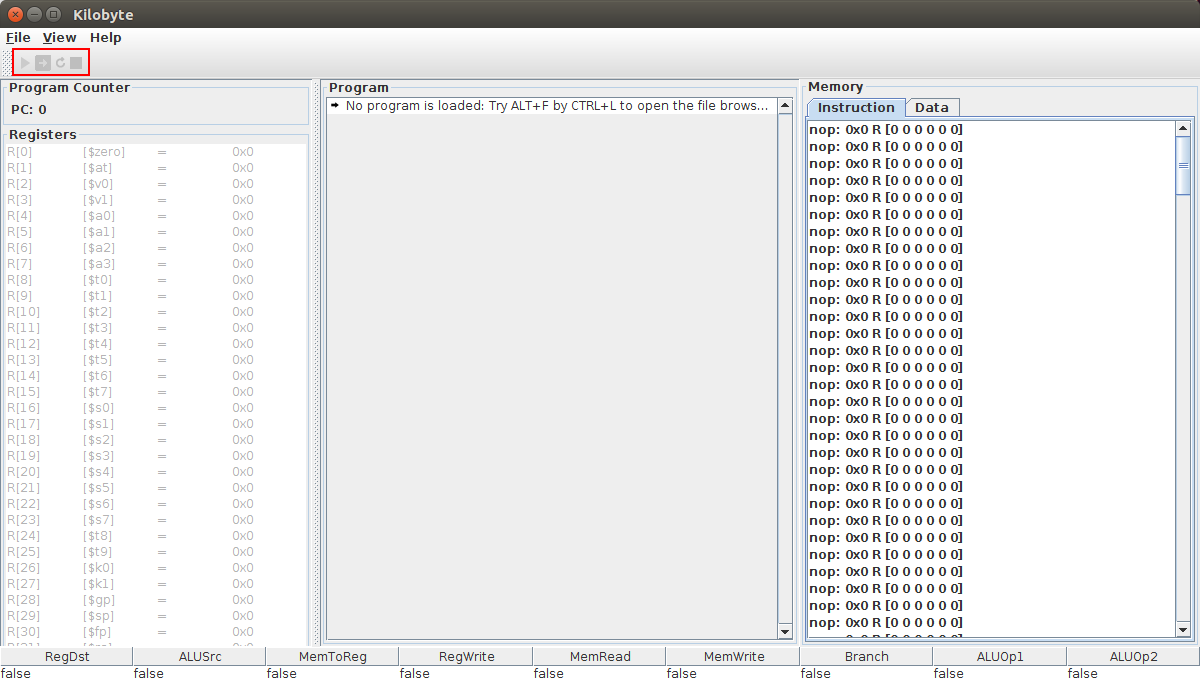
\includegraphics[width=\textwidth]{images/initial_gui_controls.png} 
  \caption{The Simulator controls are inactive at first} 
  \label{fig:inactive-controls}
\end{figure}

After loading a program through the \emph{File} menu the pertinent
controls become active. Initially two remain greyed out: "reset" and
"stop". "Stop" only becomes active once the green "play" button has been
clicked. The controls are highlighted in ~\autoref{fig:active-controls}.

\begin{figure}[H]
  \centering
  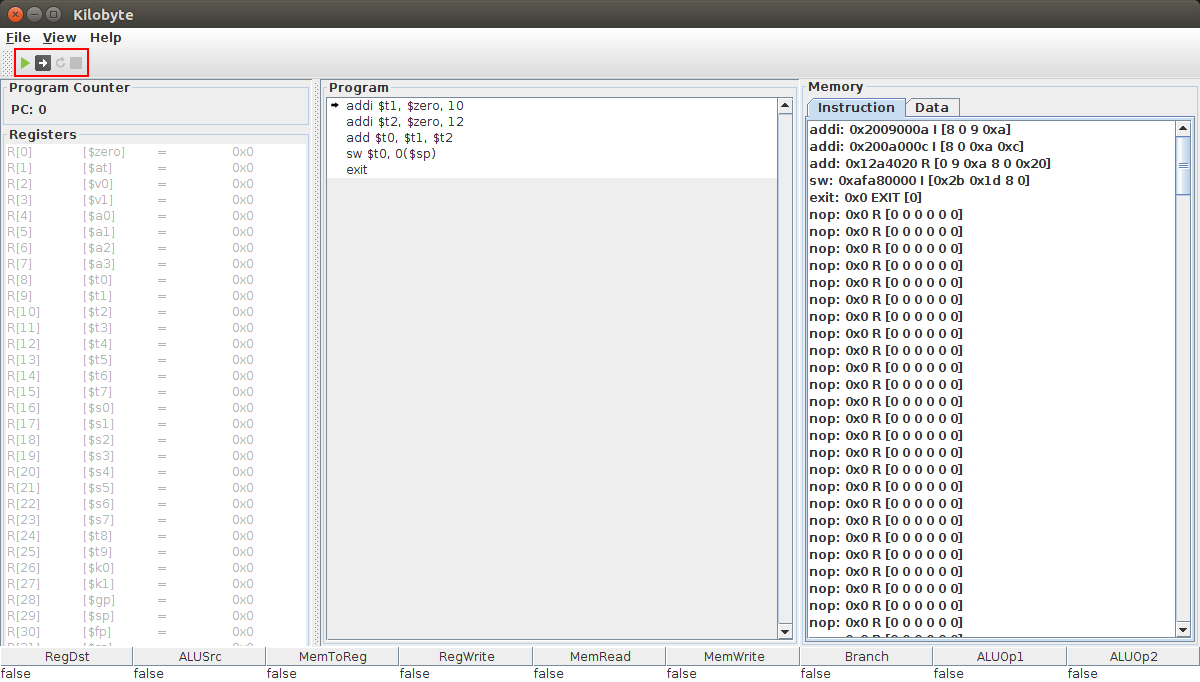
\includegraphics[width=\textwidth]{images/loaded_sw_controls.png} 
  \caption{The Simulator controls become active once a file has been loaded} 
  \label{fig:active-controls}
\end{figure}

By hovering over an instruction we get a brief description of it as
well as a sample mnemonic- and numeric representation as shown in
~\autoref{fig:tooltip}

\begin{figure}[H]
  \centering
  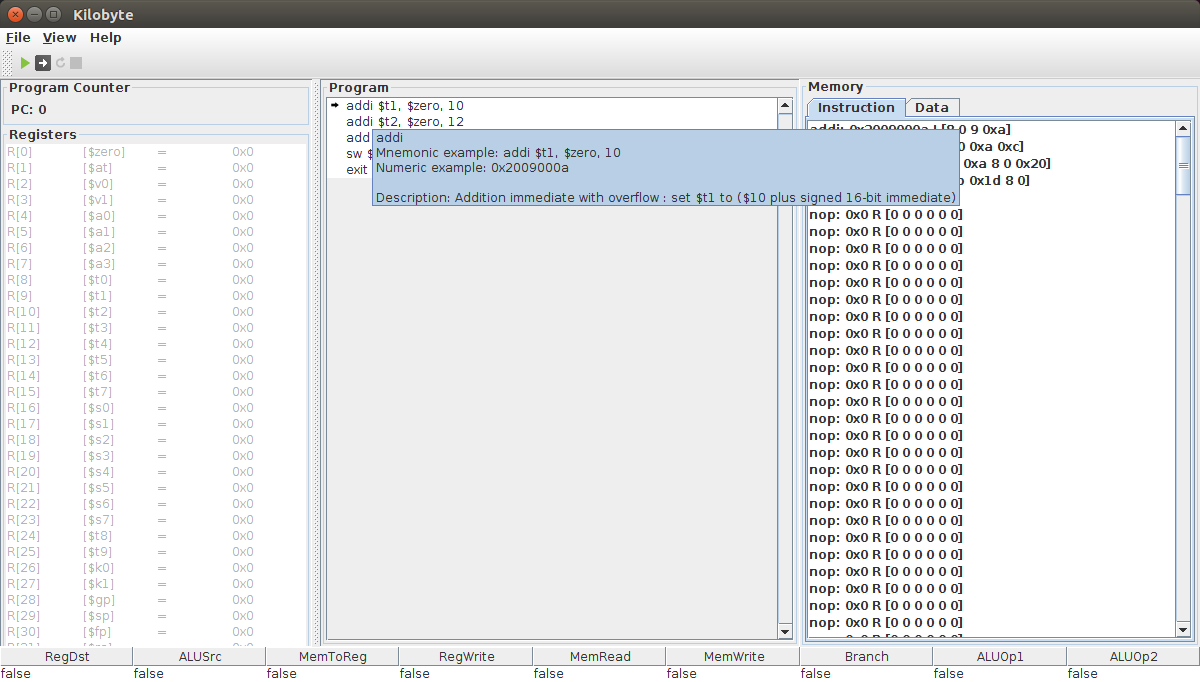
\includegraphics[width=\textwidth]{images/mouse_over_tooltip.png} 
  \caption{Tooltip} 
  \label{fig:tooltip}
\end{figure}

By clicking the "step" button we trigger the simulator to execute a
single instruction. In ~\autoref{fig:executed-addi} the step forward
icon has been highlighted and all of the changes that occurred have
been highlighted as well. We note that the control lines at the bottom
have been updated, that modified registers have been made bold, that
the program counter has been incremented to 4 and that the arrow
indicating the current instruction has stepped forward.

\begin{figure}[H]
  \centering
  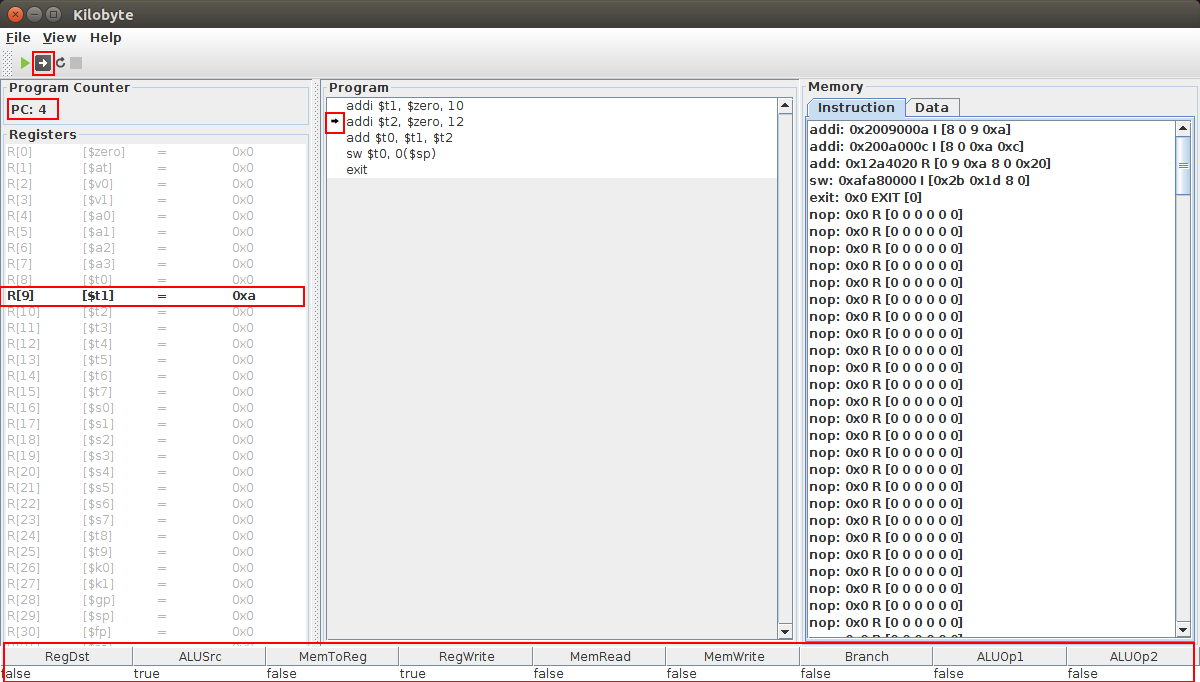
\includegraphics[width=\textwidth]{images/modified_registers_are_emboldened.png} 
  \caption{After the simulator has executed \texttt{addi}} 
  \label{fig:executed-addi}
\end{figure}

\autoref{fig:datamemory-is-bold-too} shows that data memory is also
shown in bold text once it has been modified and that all modified
registers during the lifetime of the simulation are highlighted.

\begin{figure}[H]
  \centering
  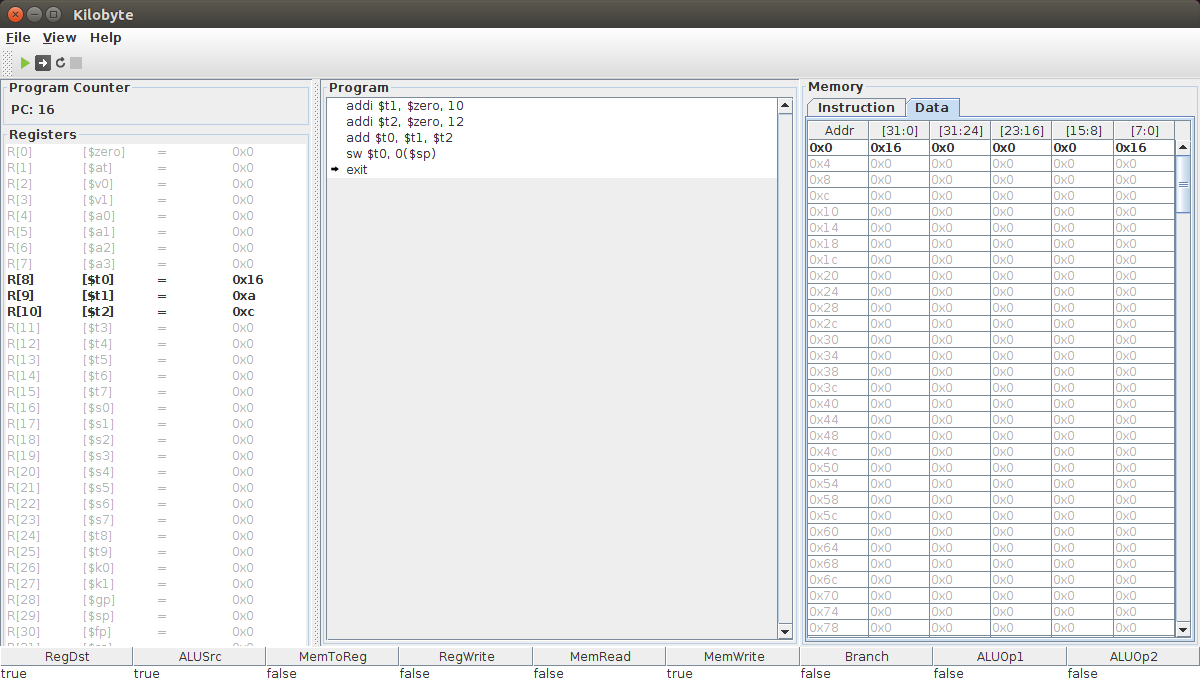
\includegraphics[width=\textwidth]{images/data_memory_is_also_emboldened.png} 
  \label{fig:datamemory-is-bold-too}
\end{figure}


\section{Software architecture}

In this section the software for the simulator is described. The
program is following the concept of the MIPS architecture, using
classes for components.

\begin{figure}[h]
    \centering
    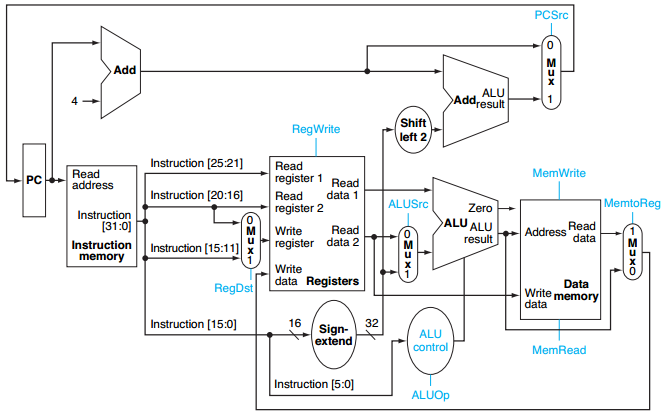
\includegraphics[scale=0.6]{datapath-r-format}
    \caption{MIPS representation\cite{Patterson:2008:COD:1502247} of the data path on R-formatted Instruction}
    \label{fig:datapathBranchOnEqual}
\end{figure}

\subsection{Simulator}
The class \texttt{Simulator} control the signals between the different components.

When an Instruction is fetched and executed, the method
\texttt{execute} is called. The following flow can be described for an
\emph{R-format} Instruction with op-code 0:


\begin{enumerate}
\item The PC will be incremented (current + 4).
\item ALU Controller will be called with the OpCode (True values:\emph{regDst, regWrite, aluOp1}).
\item Requested read-register from the Instruction is fetched from the \texttt{Register memory} is be called.
\item The fetched registers value will be sent to the ALU.
\item The output of the ALU will be saved in a register.
\end{enumerate}

The \texttt{Simulator} is the only class that can not be translated
into a component of the MIPS architecture but should be seen as the
signals that is sent between the components. It will also take care of
\texttt{MUX} conditions and the \texttt{Shift left 2} components.


\subsubsection{Component PC}

The component \texttt{Program Counter} is the class \texttt{PC}. The
class responsibility is to know what Instruction that will be read and
executed next. Each instruction size is 4 byte in the
\texttt{Instruction Memory} so a increment will be \emph{current value
  + 4}.

\subsubsection{Component Instruction Memory}

The class \texttt{InstructionMemory} consist of all Instruction given
to the simulator, the \texttt{PC} will point to an Instruction in the
memory. The number of Instruction that will be possible can be
initilized with any given size, if no size is given then it will
automatically be able to save 250 Instruction, consisting of 4 bytes
(32 bits) each, i.e. 1000 bytes.

\newpage

\subsubsection{Component ALU Controller}

The \texttt{ALU controller} is represented as the Java class
\texttt{Control}. The class state is declared in booleans which in the
MIPS architecture is called \emph{control signals} , the state is
altered by calling the method \texttt{updateOperationType}. The method
takes an parameter with the opcode that consist of six bits. The bits
will be checked towards a truth table where the state is
determined. Each state will affect the in the architecture.

\begin{table}[H]
\centering
\begin{tabular}{l|cccccc}
\hline
\bf{Opcode}    &\bf{[000000]}&\bf{[100011]} &\bf{[101011]}  &\bf{[000100]}  &\bf{[001000]}  &\bf{[001101]} \\\hline
   regDst      &   T         &   F          &   X           &   X           &   F           &   F    \\\hline
   aluSrc      &   F         &   T          &   T           &   F           &   T           &   T    \\\hline
   memtoReg    &   F         &   T          &   X           &   X           &   T           &   T    \\\hline
   regWrite    &   T         &   T          &   F           &   F           &   F           &   F    \\\hline
   memRead     &   F         &   T          &   F           &   F           &   F           &   F    \\\hline
   memWrite    &   F         &   F          &   T           &   F           &   F           &   F    \\\hline
   branch      &   F         &   F          &   F           &   T           &   F           &   F    \\\hline
   aluOp1      &   T         &   F          &   F           &   F           &   F           &   T    \\\hline
   aluOp0      &   F         &   F          &   F           &   T           &   F           &   F    \\\hline
\end{tabular}
\caption{State of the Control class is decided by the opCode received to the method \texttt{updateOperationType}}
\label{table:AluControlState}
\end{table}

As seen in Table \ref{table:AluControlState} the truth table can
affect each control signal differently. An R-format with the opCode
[000000] will make it possible for simulator to write to the register
by the control signal \emph{regDst} and \emph{regWrite}. Also will the
control signal \emph{aluOp1} change the behavior of the
\texttt{ALUOperation}, seen in section \ref{sec:ALuOperation}.Since
the state of the class is controlling the \emph{control signals} the
communication will go between \texttt{Controller} and
\texttt{Simulator}

\subsubsection{Component ALU Operation}
\label{sec:ALuOperation}

The \texttt{ALU} named \texttt{ALUOperation} makes the arithmetic
operations from given registers and, if needed, store or load from the
\texttt{Data Memory}. Given the indata to the ALU, it will preform
different operations.

\begin{table}[H]
\centering
\begin{tabular}{ccc|l}
AluOp1&AluOp2   &funct      &Operation  \\\hline
1     & 0     & \texttt{100111}     &NOR         \\\hline
1     & 0     & \texttt{000010}     &SRL         \\\hline
1     & 0     & \texttt{000011}     &SRA         \\\hline
1     & X     & \texttt{XX0010}     &SUBTRACT    \\\hline
1     & 0     & \texttt{XX0000}     &ADD         \\\hline
1     & 0     & \texttt{XX0100}     &AND         \\\hline
1     & 0     & \texttt{XX0101}     &OR          \\\hline
1     & X     & \texttt{XX1010}     &SLT         \\\hline
0     & 0     & \texttt{XXXXXX}     &ADD         \\\hline
0     & 1     & \texttt{XXXXXX}     &SUBTRACT    \\\hline
1     & 0     & \texttt{XXXXXX}     &OR          \\\hline
\end{tabular}
\caption{ALU operation depending on what AluOp set in \texttt{Controller} and funct-field.}
\label{tab:ALUoperation}
\end{table}

As shown in table \ref{tab:ALUoperation} depending on the
\texttt{AluOp1} and \texttt{AluOp2} that are set in the
\texttt{Controller} but also the funct-field in the Instruction.

\subsubsection{Component SignExtender}

The component as well as the class \texttt{SignExtender} will take a
given value and extend it. For the purpose in MIPS it will take a 16
bits value and transform it to a 32 bit. This is used on \texttt{jump}
and \texttt{branch} Instructions.

\subsubsection{Component Data Memory}

The \texttt{DataMemory} class concist of 1000 \texttt{ByteBuffer}s to
simulate the Data memory in the MIPS architecture.


\clearpage

\printbibliography

\end{document}
